\chapterbackmatter{Solutions to Supplementary Exercises}

\begin{enumerate}
\SupplementarySolution{1}{Positive Spectral Measures, Pole Weights, and Sum Rules}
\begin{enumerate}
\item
Translation invariance gives
\[
 \bra{\Omega}\phi(x)\ket{n,p}
 =e^{ip\cdot x}\bra{\Omega}\phi(0)\ket{n,p}.
\]
Inserting the identity and collecting states with the same invariant mass
therefore yields
\[
 \bra{\Omega}\phi(x)\phi(0)\ket{\Omega}
 =\int_0^\infty d\mu^2\,\rho(\mu^2)
 \Delta_+(x;\mu^2),
\]
where, schematically,
\[
 \rho(\mu^2)=
 \sum_n(2\pi)^3\delta(\mu^2-\mu_n^2)
 \left|\bra{\Omega}\phi(0)\ket n\right|^2 .
\]
The omitted factors are just those fixed by the chosen invariant
normalization.  Every summand is an absolute square, so
\(\rho(\mu^2)\geq0\).  If a stable particle of mass \(m\) has
\(\bra{\Omega}\phi(0)\ket p\neq0\), its orbit under translations produces
\[
 \rho(\mu^2)\supset Z\delta(\mu^2-m^2),\qquad Z>0.
\]
All states with continuously variable relative momenta contribute a
nonnegative continuum rather than an isolated delta function.
\item
The one-particle contribution and the continuum separate as
\[
 \rho(\mu^2)=Z\delta(\mu^2-m^2)
 +\theta(\mu^2-M_{\rm th}^2)\rho_c(\mu^2),
\qquad \rho_c\geq0.
\]
Thus
\[
 D(p)=\frac{Z}{p^2+m^2-i0}
 +\int_{M_{\rm th}^2}^{\infty}
 \frac{\rho_c(\mu^2)\,d\mu^2}{p^2+\mu^2-i0}.
\]
There is an isolated simple pole at \(p^2=-m^2\), with positive residue
\(Z\).  The continuum produces a branch point at
\(p^2=-M_{\rm th}^2\) and a cut extending along the timelike axis.  The
assumption of stability means \(m<M_{\rm th}\); otherwise the pole lies on
the cut and generally moves away from the physical sheet, describing a
resonance rather than an asymptotic particle.
\item
The spectral commutator is
\[
 \bra{\Omega}[\phi(x),\phi^\dagger(y)]\ket{\Omega}
 =\int_0^\infty d\mu^2\,\rho(\mu^2)
 \bigl[\Delta_+(x-y;\mu^2)-\Delta_+(y-x;\mu^2)\bigr].
\]
Differentiate with respect to \(x^0\) and set \(x^0=y^0\).  For every
\(\mu\), the bracket on the right gives
\(-i\delta^3(\mathbf x-\mathbf y)\).  Comparing with the canonical
commutator gives
\[
 \boxed{\int_0^\infty\rho(\mu^2)\,d\mu^2=1.}
\]
Writing
\(\rho=Z\delta(\mu^2-m^2)+\rho_c\) and using
\(\rho_c\geq0\) gives
\[
 1=Z+\int\rho_c,\qquad 0\leq Z\leq1.
\]
The statement concerns a regulated, canonically normalized bare field.
For a renormalized field the right-hand side is rescaled with the field
normalization.
\end{enumerate}

\SupplementarySolution{2}{The Thermal Lehmann Representation}
Choose simultaneous energy--momentum eigenstates,
\[
 H\ket n=E_n\ket n,
 \qquad \mathbf P\ket n=\mathbf p_n\ket n,
\]
and define
\[
 O_{nm}=\bra nO(0)\ket m,qquad
 \omega_{mn}=E_m-E_n,qquad
 \mathbf q_{mn}=\mathbf p_m-\mathbf p_n.
\]
For Hermitian \(O\), inserting a complete set on each side of the time
ordering and interchanging \(n\) and \(m\) in the negative-time term gives
\[
 \begin{split}
 -iD_\beta(t,\mathbf x)
 =\frac1{Z_\beta}\sum_{n,m}|O_{nm}|^2
 e^{-i\omega_{mn}t+i\mathbf q_{mn}\cdot\mathbf x}
 \bigl[\theta(t)e^{-\beta E_n}
 +\theta(-t)e^{-\beta E_m}\bigr].
 \end{split}
\]
This is already the thermal Lehmann representation in position space.
With the Fourier convention
\(F(\omega,\mathbf p)=\int d^4x\,
e^{i\omega t-i\mathbf p\cdot\mathbf x}F(x)\), it becomes
\[
 \begin{split}
 -iD_\beta(\omega,\mathbf p)
 ={}&\frac{i}{Z_\beta}\sum_{n,m}(2\pi)^3
 \delta^3(\mathbf p-\mathbf q_{mn})|O_{nm}|^2\\
 &\times\left[
 \frac{e^{-\beta E_n}}{\omega-\omega_{mn}+i0}
 -\frac{e^{-\beta E_m}}{\omega-\omega_{mn}-i0}
 \right].
 \end{split}
\]

It is useful to separate the two thermal Wightman functions.  Their common
positive-frequency weight and the commutator spectral function are
\[
 \begin{split}
 G_\beta^>(\omega,\mathbf p)
 &\equiv\frac{(2\pi)^4}{Z_\beta}\sum_{n,m}e^{-\beta E_n}
 |O_{nm}|^2\delta(\omega-\omega_{mn})
 \delta^3(\mathbf p-\mathbf q_{mn}),\\
 \rho_\beta(\omega,\mathbf p)
 &\equiv\frac{(2\pi)^4}{Z_\beta}\sum_{n,m}
 \bigl(e^{-\beta E_n}-e^{-\beta E_m}\bigr)|O_{nm}|^2
 \delta(\omega-\omega_{mn})
 \delta^3(\mathbf p-\mathbf q_{mn}).
 \end{split}
\]
Since \(E_m=E_n+\omega\) on the support of the delta function,
\[
 G_\beta^<(\omega,\mathbf p)
 =e^{-\beta\omega}G_\beta^>(\omega,\mathbf p),
 \qquad
 \rho_\beta=(1-e^{-\beta\omega})G_\beta^>.
\]
This is detailed balance, or the frequency-space KMS relation.  In terms of
\(n_B(\omega)=(e^{\beta\omega}-1)^{-1}\), the time-ordered answer may also
be written
\[
 -iD_\beta(\omega,\mathbf p)
 =i\int_{-\infty}^{\infty}\frac{d\omega'}{2\pi}\,
 \rho_\beta(\omega',\mathbf p)
 \left[
 \frac{1+n_B(\omega')}{\omega-\omega'+i0}
 -\frac{n_B(\omega')}{\omega-\omega'-i0}
 \right].
\]
The heat bath selects a rest frame, so the thermal density depends
separately on \(\omega\) and \(\mathbf p\), rather than only on a Lorentz
invariant mass.

Assume a unique vacuum with \(E_0=0\).  As \(\beta\to\infty\), only
\(n=0\) survives in the positive-time term and only \(m=0\) in the
negative-time term.  Thus
\[
 \begin{split}
 -iD(\omega,\mathbf p)=i\sum_m(2\pi)^3\Bigg[
 &\frac{|O_{0m}|^2\delta^3(\mathbf p-\mathbf p_m)}
       {\omega-E_m+i0}\\
 &-\frac{|O_{m0}|^2\delta^3(\mathbf p+\mathbf p_m)}
       {\omega+E_m-i0}\Bigg],
 \end{split}
\]
which is the usual vacuum Lehmann representation; Lorentz invariance then
reorganizes the intermediate states into the standard invariant-mass
spectral density.

\SupplementarySolution{3}{Local and Momentum-Space Ward--Takahashi Identities}
\begin{enumerate}
\item
Perform the infinitesimal change of variables
\[
 \delta\Phi=i q\alpha(x)\Phi,\qquad
 \delta\Phi^\dagger=-iq\alpha(x)\Phi^\dagger.
\]
Invariance of the functional measure and integration by parts in the
action give a term
\(-\int d^4x\,\alpha\,\partial_\mu j^\mu\).  Variation of the inserted
fields gives delta functions at their positions.  Removing the arbitrary
\(\alpha(x)\) yields
\[
 \boxed{
 \begin{aligned}
 \partial_\mu^x
 \langle Tj^\mu(x)\Phi(y)\Phi^\dagger(z)\rangle
 ={}&-q\delta^4(x-y)
       \langle T\Phi(y)\Phi^\dagger(z)\rangle\\
 &+q\delta^4(x-z)
       \langle T\Phi(y)\Phi^\dagger(z)\rangle .
 \end{aligned}}
\]
The relative signs reflect the opposite charges of \(\Phi\) and
\(\Phi^\dagger\).  The same result follows from differentiating the
step functions in the operator time ordering.
\item
Let \(q=\ell-k\), and define the connected three-point function by
\[
 G^\mu(k,\ell)
 =-iq\,\Delta'(k)\Gamma^\mu(k,\ell)\Delta'(\ell).
\]
Fourier transformation of the two contact terms in the local identity
gives the difference of full propagators.  After cancelling the common
charge and amputating both scalar legs,
\[
 \boxed{\;
 q_\mu\Gamma^\mu(k,\ell)
 =i\Delta'^{-1}(k)-i\Delta'^{-1}(\ell).\;}
\]
For the free inverse propagator \(k^2+m^2\), the vertex
\(-i(k+\ell)^\mu\) gives
\(q_\mu\Gamma^\mu=i(k^2-\ell^2)\), exactly the required difference.
The equality therefore holds for the fully dressed quantities with the
same convention.
\item
Set \(\ell=k+q\), expand for small \(q\), and retain the linear term:
\[
 q_\mu\Gamma^\mu(k,k)
 =-i q_\mu\frac{\partial}{\partial k_\mu}
 \Delta'^{-1}(k)+O(q^2).
\]
Because \(q_\mu\) is arbitrary,
\[
 \boxed{\Gamma^\mu(k,k)
 =-i\frac{\partial\Delta'^{-1}(k)}{\partial k_\mu}.}
\]
Near the pole, the coefficient multiplying \(k^2+m^2\) in the inverse
propagator is the field-strength normalization.  The same coefficient
appears in the zero-momentum vertex through the derivative formula.
Consequently the ultraviolet counterterms multiplying the charged-field
kinetic term and the one-photon vertex are tied; in standard notation the
Ward identity enforces \(Z_1=Z_2\).
\end{enumerate}

\SupplementarySolution{4}{Charge Conjugation and Odd-Photon Selection Rules}
\begin{enumerate}
\item
Set
\[
 F_{\mu\nu}=\partial_\mu A_\nu-\partial_\nu A_\mu,
 \qquad D_\mu=\partial_\mu+ieA_\mu.
\]
In the volume's mostly-plus convention the two Lagrangians are
\[
 \boxed{\mathcal L_{\mathrm{SQED}}
 =-\frac14F_{\mu\nu}F^{\mu\nu}
 -(D_\mu\phi)^\dagger D^\mu\phi-M^2\phi^\dagger\phi,}
\]
\[
 \boxed{\mathcal L_{\mathrm{QED}}
 =-\frac14F_{\mu\nu}F^{\mu\nu}
 -\bar\psi(\gamma^\mu D_\mu+m)\psi.}
\]
They are invariant under
\[
 A_\mu\longmapsto A_\mu+\partial_\mu\Lambda,qquad
 \phi\longmapsto e^{-ie\Lambda}\phi,qquad
 \psi\longmapsto e^{-ie\Lambda}\psi,
\]
because \(D_\mu\phi\) and \(D_\mu\psi\) acquire the same phase as their
fields and \(F_{\mu\nu}\) is unchanged.

For a constant phase \(\varepsilon=e\Lambda\), so that
\(\delta\phi=-i\varepsilon\phi\) and
\(\delta\psi=-i\varepsilon\psi\), the unit-normalized Noether currents are
\[
 \boxed{J_\phi^\mu
 =-i\bigl[\phi^\dagger D^\mu\phi
 -(D^\mu\phi)^\dagger\phi\bigr],
 \qquad
 J_\psi^\mu=i\bar\psi\gamma^\mu\psi.}
\]
Multiplication by the coupling gives the corresponding gauge-source
normalization.  The Euler--Lagrange equations give
\(\partial_\mu J_\phi^\mu=\partial_\mu J_\psi^\mu=0\).
\item
Charge conjugation must send
\[
 \boxed{\widehat C^{-1}A_\mu\widehat C=-A_\mu.}
\]
Indeed, it then maps
\[
 D_\mu\phi\longmapsto
 (\partial_\mu-ieA_\mu)\phi^\dagger=(D_\mu\phi)^\dagger,
 \qquad F_{\mu\nu}\longmapsto-F_{\mu\nu}.
\]
Both the Maxwell term and every scalar term are therefore invariant.  The
same calculation gives
\(\widehat C^{-1}J_\phi^\mu\widehat C=-J_\phi^\mu\).
\item
The supplied matrix identities imply \(\mathsf C^2=-\mathbf1\) and
\(\mathsf C(\gamma^\mu)^{\mathsf T}\mathsf C=\gamma^\mu\).  Therefore
\[
 \begin{split}
 \widehat C^{-1}(\bar\psi\psi)\widehat C
 &=\psi^{\mathsf T}\mathsf C^2\bar\psi^{\mathsf T}
 =-\psi^{\mathsf T}\bar\psi^{\mathsf T}=\bar\psi\psi,\\
 \widehat C^{-1}(\bar\psi\gamma^\mu\psi)\widehat C
 &=\psi^{\mathsf T}\mathsf C\gamma^\mu\mathsf C\bar\psi^{\mathsf T}
 =-\bar\psi(\mathsf C\gamma^\mu\mathsf C)^{\mathsf T}\psi
 =-\bar\psi\gamma^\mu\psi.
 \end{split}
\]
For the kinetic term the same Grassmann rearrangement gives
\[
 \bar\psi^C\gamma^\mu\partial_\mu\psi^C
 =-(\partial_\mu\bar\psi)\gamma^\mu\psi
 =\bar\psi\gamma^\mu\partial_\mu\psi
 -\partial_\mu(\bar\psi\gamma^\mu\psi).
\]
It is invariant in the action.  The interaction is invariant because both
\(A_\mu\) and \(\bar\psi\gamma^\mu\psi\) are odd, while the mass and Maxwell
terms are even.  Hence \(\mathcal L_{\mathrm{QED}}\) is charge-conjugation
invariant up to the displayed total derivative, and
\(\widehat C^{-1}J_\psi^\mu\widehat C=-J_\psi^\mu\).
\item
Let \(X_i\) be either \(A^{\mu_i}(x_i)\) or \(J^{\mu_i}(x_i)\).  Since the
vacuum and the time-ordering operation are invariant,
\[
 \begin{split}
 \bra\Omega T\{X_1\cdots X_n\}\ket\Omega
 &=\bra\Omega\widehat C^{-1}T\{X_1\cdots X_n\}\widehat C\ket\Omega\\
 &=(-1)^n\bra\Omega T\{X_1\cdots X_n\}\ket\Omega.
 \end{split}
\]
For odd \(n\) the correlator equals its negative and must vanish.  This is
an exact operator argument, so it is valid to all orders rather than merely
diagram by diagram.  LSZ reduction then says that any amplitude having an
odd number of external photons and no charged external particles vanishes:
three-photon scattering or splitting is forbidden, while even-photon
light-by-light scattering is not.  Perturbatively this is Furry's theorem,
the cancellation between the two orientations of each charged loop with an
odd number of photon attachments.
\end{enumerate}

\SupplementarySolution{5}{Current Conservation after LSZ Reduction}
The divergence of the current correlator is a sum of terms in which the
current point is collapsed onto one charged-field insertion.  Such a term
has one fewer independent spacetime point and therefore lacks the complete
set of simultaneous one-particle poles required by LSZ for the original
process.  Multiplying by every external inverse propagator and taking all
mass-shell limits annihilates it.

An external photon contributes a polarization contraction
\(\epsilon_\mu\mathcal M^\mu\).  Replacing
\(\epsilon_\mu\) by its momentum turns the current insertion into its
Fourier-space divergence.  The preceding pole argument then gives
\[
 \boxed{k_\mu\mathcal M^\mu=0.}
\]
The assertion applies to the gauge-invariant sum of diagrams; an individual
diagram need not contain all contact-term cancellations.

\SupplementarySolution{6}{Two Form Factors for an Elastic Dirac Current and Charge and Magnetic Moment at Zero Transfer}
\begin{enumerate}
\item
For \(q=p'-p\), parity permits only vector bilinears.  The Dirac equations
and the Gordon identity reduce all candidates to
\[
 \boxed{\;
 \Gamma^\mu(q)=
 \gamma^\mu F_1(q^2)
 +\frac{i\sigma^{\mu\nu}q_\nu}{2m}F_2(q^2).\;}
\]
Both terms are conserved between equal-mass on-shell spinors.  Using
\[
 \bar u'\,i\sigma^{\mu\nu}q_\nu u
 =\bar u'\bigl(2m\gamma^\mu-(p'+p)^\mu\bigr)u
\]
in the conventional gamma-matrix normalization gives the equivalent basis
\[
 \bar u'\Gamma^\mu u
 =\bar u'\left[
 \gamma^\mu(F_1+F_2)
 -\frac{(p'+p)^\mu}{2m}F_2
 \right]u.
\]
Factors of \(i\) move between the Gordon identity and the coefficient
functions in the volume's mostly-plus convention, but the two independent
scalar functions and all observables are unchanged.
\item
In the nonrelativistic expansion, the temporal current is
\[
 J^0=e\,F_1(0)\,\chi'^\dagger\chi+O(|\mathbf q|/m),
\]
so charge normalization gives \(F_1(0)=Q\) when the overall coupling is
\(e\).  The spatial current contains
\[
 \mathbf J_{\rm spin}
 =\frac{e}{2m}\,[F_1(0)+F_2(0)]\,
 \chi'^\dagger i\mathbf q\times\boldsymbol\sigma\,\chi .
\]
Hence
\[
 \boxed{\boldsymbol\mu
 =\frac{e}{2m}[F_1(0)+F_2(0)]\boldsymbol\sigma.}
\]
For a minimally coupled point Dirac particle at tree level,
\(F_1(0)=Q\) and \(F_2(0)=0\); for \(Q=1\), this is the Dirac value
\(g=2\).  Radiative corrections appear as the anomalous Pauli form factor
\(F_2(0)\).
\end{enumerate}

\SupplementarySolution{7}{Why a Transition Charge Must Vanish and Opposite-Parity Electromagnetic Transitions}
\begin{enumerate}
\item
A useful conserved basis for unequal masses is
\[
 \bar u_2\left[
 \left(\gamma^\mu-\frac{q^\mu\slashed q}{q^2}\right)F_T(q^2)
 +\frac{i\sigma^{\mu\nu}q_\nu}{m_1+m_2}G_T(q^2)
 \right]u_1 .
\]
Contracting with \(q_\mu\) annihilates both structures identically.  The
first, however, contains \(q^\mu/q^2\).  Since
\[
 \bar u_2\slashed q\,u_1
 =i(m_2-m_1)\bar u_2u_1
\]
does not vanish for \(m_2\ne m_1\), absence of a kinematic pole at
\(q^2=0\) requires
\[
 \boxed{F_T(0)=0.}
\]
Equivalently, the zero-momentum charge operator commutes with the
Hamiltonian and cannot connect energy eigenstates of different mass.
\item
A vector current between opposite-parity states must be represented by an
axial-looking spinor bilinear:
\[
 \bar u_2\left[
 \gamma^\mu\widetilde F+P^\mu\widetilde G
 +q^\mu\widetilde H\right]\gamma_5u_1 .
\]
Anticommuting \(\gamma_5\) through the initial Dirac equation gives
\[
 \bar u_2\slashed q\gamma_5u_1
 =i(m_2+m_1)\bar u_2\gamma_5u_1.
\]
Therefore current conservation reads
\[
 i(m_2+m_1)\widetilde F
 -(m_2^2-m_1^2)\widetilde G
 +q^2\widetilde H=0.
\]
The sum appears because \(\gamma_5\) reverses the sign of the initial
\(\slashed p_1\).  A manifestly transverse basis is obtained by multiplying
  the two structures of the preceding part by \(\gamma_5\), and its
transition-charge coefficient again vanishes at \(q^2=0\).
\end{enumerate}

\SupplementarySolution{8}{The Scalar Charge-Radius Expansion and Transverse Decomposition of Vacuum Polarization}
\begin{enumerate}
\item
For equal scalar masses, covariance gives
\[
 \bra{p'}J^\mu(0)\ket p
 =\mathcal N\bigl[(p'+p)^\mu F(q^2)+q^\mu H(q^2)\bigr].
\]
Because \(q\cdot(p'+p)=p'^2-p^2=0\), conservation requires
\(q^2H=0\), and regularity gives \(H=0\).  Charge normalization fixes
\[
 F(0)=1.
\]
In the Breit frame, \(q^0=0\) and the Fourier transform of the static
charge distribution is \(F(\mathbf q^2)\).  Its small-\(\mathbf q\)
expansion is
\[
 \boxed{\;
 F(q^2)=1-\frac16\langle r^2\rangle q^2+O(q^4),
 \qquad
 \langle r^2\rangle=-6F'(0),\;}
\]
where \(q^2=\mathbf q^2>0\) in the volume's mostly-plus convention.
\item
The most general symmetric rank-two function is
\[
 \Pi^{\mu\nu}(q)=A(q^2)\eta^{\mu\nu}
 +B(q^2)q^\mu q^\nu.
\]
The Ward identity gives \(A+q^2B=0\), hence
\[
 \boxed{\Pi^{\mu\nu}(q)
 =(q^2\eta^{\mu\nu}-q^\mu q^\nu)\pi(q^2).}
\]
Dyson summation changes the transverse photon denominator from \(q^2\) to
\(q^2[1-\pi(q^2)]\), up to the convention used for the sign of
\(\Pi\).  The explicit factor \(q^2\) remains.  If the renormalized
\(\pi(q^2)\) is finite at the origin and its residue is normalized by
\(\pi(0)=0\), the propagator retains a pole at \(q^2=0\) with the chosen
unit transverse residue: radiative corrections do not generate a photon
mass.
\end{enumerate}

\SupplementarySolution{9}{Subtracted Dispersion Relations and Positivity}
\begin{enumerate}
\item
Apply Cauchy's theorem to
\[
 \frac{F(\zeta)}{(\zeta-z)(\zeta-z_0)}
\]
and collapse the contour around the cut.  Real analyticity gives
\(\operatorname{Disc}F(s)=2i\operatorname{Im}F(s+i0)\).  The result is
\[
 \boxed{\;
 F(z)=F(z_0)+\frac{z-z_0}{\pi}
 \int_{s_0}^{\infty}
 \frac{\operatorname{Im}F(s+i0)\,ds}
 {(s-z_0)(s-z-i0)}.\;}
\]
One subtraction is sufficient because the extra denominator makes the
large-circle contribution vanish when \(F\) grows no faster than a
constant.  The formula reproduces \(F(z_0)\) identically and has the
required discontinuity on the cut.
\item
After \(n\) subtractions, the contour integrand behaves on a large circle
as \(F(\zeta)/\zeta^{n+1}\).  Its arc integral therefore scales as
\(R^{N-n}\log R\).  A sufficient condition for it to vanish is
\[
 \boxed{n>N.}
\]
Thus \(n=N+1\) subtractions suffice for the stated bound.  The general
answer is
\[
 F(z)=P_{n-1}(z)
 +\frac{(z-z_0)^n}{\pi}\int_{s_0}^{\infty}
 \frac{\operatorname{Im}F(s)\,ds}
 {(s-z_0)^n(s-z-i0)}.
\]
Changing \(z_0\) rearranges the first \(n\) Taylor data into a different
polynomial \(P_{n-1}\).  The integral's discontinuity remains
\(2i\operatorname{Im}F\), so two subtraction prescriptions differ only by
an entire polynomial of degree at most \(n-1\).
\item
For one subtraction at \(z_0<s_0\),
\[
 F^{(n)}(z_0)=\frac{n!}{\pi}
 \int_{s_0}^{\infty}
 \frac{\operatorname{Im}F(s)\,ds}{(s-z_0)^{n+1}},
 \qquad n\geq1.
\]
Every denominator is positive, so a nonnegative absorptive part makes all
these derivatives nonnegative.  In particular the asserted inequalities
hold for \(n\geq2\).

There is a qualification for the first derivative.  If the actual
high-energy behavior requires two or more subtractions, a free linear
polynomial is present; then \(F'(z_0)\) contains an undetermined subtraction
constant, while derivatives above the polynomial's degree remain dispersive
and positive.  If a genuinely once-subtracted relation is justified, the
displayed formula also proves \(F'(z_0)\geq0\).
\end{enumerate}

\SupplementarySolution{10}{Muon Vacuum Polarization from the Optical Theorem}
\begin{enumerate}
\item
The required graph is the forward \(s\)-channel photon exchange with a
muon loop inserted into the photon line:
\begin{center}
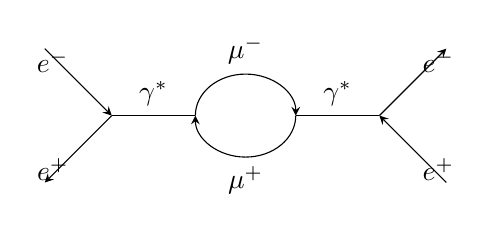
\begin{tikzpicture}[x=0.85cm,y=0.85cm,>=stealth]
 \draw[->] (-3,1)--(-2,0) node[midway,above left] {\(e^-\)};
 \draw[<-] (-3,-1)--(-2,0) node[midway,below left] {\(e^+\)};
 \draw (-2,0)--(-0.75,0) node[midway,above] {\(\gamma^*\)};
 \draw[->] (-0.75,0) arc (180:0:0.75 and 0.62)
   node[midway,above] {\(\mu^-\)};
 \draw[->] (0.75,0) arc (0:-180:0.75 and 0.62)
   node[midway,below] {\(\mu^+\)};
 \draw (0.75,0)--(2,0) node[midway,above] {\(\gamma^*\)};
 \draw[->] (2,0)--(3,1) node[midway,above right] {\(e^-\)};
 \draw[<-] (2,0)--(3,-1) node[midway,below right] {\(e^+\)};
\end{tikzpicture}
\end{center}
Write the transverse muon contribution as
\[
 \Pi_\mu^{\alpha\beta}(q)
 =(q^\alpha q^\beta-q^2\eta^{\alpha\beta})\Pi_\mu(s),
 \qquad s=-q^2.
\]
Cutting the two muon propagators is equivalent to inserting the on-shell
\(\mu^+\mu^-\) states in the current two-point function.  With
\[
 \beta_\mu=\sqrt{1-\frac{4m_\mu^2}{s}},
 \qquad x_\pm=\frac12(1\pm\beta_\mu),
\]
the scalar absorptive part is
\[
 \begin{split}
 \operatorname{Im}\Pi_\mu(s+i0)
 &=\frac{Q_\mu^2}{2\pi}
   \int_{x_-}^{x_+}dx\,x(1-x)\\
 &=\boxed{\frac{Q_\mu^2}{12\pi}
 \left(1+\frac{2m_\mu^2}{s}\right)
 \sqrt{1-\frac{4m_\mu^2}{s}}\,
 \theta(s-4m_\mu^2)}.
 \end{split}
\]
Indeed, a regulator-dependent representation has the form
\[
 \Pi_\mu(s)=C_{\mathrm{UV}}
 -\frac{Q_\mu^2}{2\pi^2}\int_0^1dx\,x(1-x)
 \log\!\left[m_\mu^2-sx(1-x)-i0\right],
\]
up to a real convention-dependent additive constant.  The cutoff occurs
only in the real local term \(C_{\mathrm{UV}}\); the logarithm acquires an
imaginary part only for \(x_-<x<x_+\).  The boxed answer is consequently
cutoff independent.

For negligible electron mass, the same cut gives
\[
 \sigma(e^+e^-\to\mu^+\mu^-)
 =\frac{Q_e^2}{s}\operatorname{Im}\Pi_\mu(s+i0)
 =\frac{Q_e^2Q_\mu^2}{12\pi s}
 \left(1+\frac{2m_\mu^2}{s}\right)\beta_\mu,
\]
which identifies precisely the \(Q_e^2Q_\mu^2\) contribution to the
forward amplitude.
\item
Write \(S=\mathbf1+iT\).  Unitarity gives
\[
 -i(T-T^\dagger)=T^\dagger T,
\]
and hence the correctly conjugated matrix-element identity is
\[
 -i\bigl[\mathcal M(a\to b)-\mathcal M(b\to a)^*\bigr]
 =\sum_f\int d\Phi_f\,
 \mathcal M(b\to f)^*\mathcal M(a\to f).
\]
Thus the missing conjugation in the source display is a typographical
omission, not a changed unitarity convention.  Setting \(b=a\) gives
\[
 2\operatorname{Im}\mathcal M(a\to a)
 =\sum_f\int d\Phi_f\,|\mathcal M(a\to f)|^2\geq0.
\]
For the \(\mu^+\mu^-\) intermediate state, division by the incident flux
reproduces
\[
 \frac{Q_e^2}{s}\operatorname{Im}\Pi_\mu(s)
 =\sigma(e^+e^-\to\mu^+\mu^-)\geq0,
\]
which is the optical theorem for this cut.

In a Wick expansion, closing a chain of fermion contractions into a cycle
requires one additional odd permutation of Grassmann fields.  Each
independent closed fermion loop therefore contributes \((-1)\).  Directly
in the present example, omitting that sign reverses the cut of the loop and
would give
\(\operatorname{Im}\Pi_\mu=-Q_\mu^2\beta_\mu
(1+2m_\mu^2/s)/(12\pi)\), making the cross-section negative.  Including the
closed-loop minus sign gives the positive absorptive part above and exactly
restores unitarity.
\end{enumerate}

\SupplementarySolution{11}{The Complete Compton Trace}
Put
\[
 a=k_1\cdot k_2,
 \qquad b=k_1\cdot k_2'.
\]
Momentum conservation and the mass-shell conditions imply
\[
 k_2\cdot k_2'=a-b,
 \qquad k_1'\cdot k_2=b,
 \qquad k_1'\cdot k_2'=a,
 \qquad k_1'\cdot k_1=-m^2+a-b.
\]
These relations eliminate every scalar product generated by the trace in
favor of \(a,b,m^2\).

Denote the two numerator structures in the first parenthesis of the prompt
by \(N_s^{\mu\nu}\) and \(N_u^{\mu\nu}\), and those in the second by
\(\bar N_s^{\alpha\beta}\) and \(\bar N_u^{\alpha\beta}\), before their
denominators \(a\) and \(b\) are included.  Apply the supplied contractions
with \(d=4\), and then use
\[
 \operatorname{tr}\mathbf1=4,
 \qquad
 \operatorname{tr}(\gamma^\mu\gamma^\nu)=4\eta^{\mu\nu},
\]
and
\[
 \operatorname{tr}(\gamma^\mu\gamma^\nu\gamma^\rho\gamma^\sigma)
 =4\bigl(\eta^{\mu\nu}\eta^{\rho\sigma}
 -\eta^{\mu\rho}\eta^{\nu\sigma}
 +\eta^{\mu\sigma}\eta^{\nu\rho}\bigr).
\]
All traces with an odd number of gamma matrices vanish.  The four pieces of
the contracted trace reduce to
\[
 \begin{array}{c|c}
 \text{numerator pair}&
 \eta_{\mu\alpha}\eta_{\nu\beta}
 \operatorname{tr}\bigl[(\slashed{k}_1'+im)
 N^{\mu\nu}(\slashed{k}_1+im)\bar N^{\alpha\beta}\bigr]\\ \hline
 s\text{--}s&32(ab-m^2a+m^4)\\
 u\text{--}u&32(ab+m^2b+m^4)\\
 s\text{--}u&16m^2(a-b)-32m^4\\
 u\text{--}s&16m^2(a-b)-32m^4
 \end{array}
\]
The denominators are respectively \(a^2,b^2,ab,ab\).  Their sum is therefore
\[
 \begin{split}
 \mathcal T
 &=32\left[
 \frac ba+\frac ab
 +2m^2\left(\frac1b-\frac1a\right)
 +m^4\left(\frac1b-\frac1a\right)^2
 \right].
 \end{split}
\]
Finally Eq.~(11.46) contributes the prefactor \(e^4/4\), and the requested
unpolarized average supplies another factor \(1/4\).  Hence
\[
 \boxed{
 \frac14\sum_{\sigma,\sigma'}|\widetilde{\mathcal M}_{c}|^2
 =2e^4\left[
 \frac ba+\frac ab
 +2m^2\left(\frac1b-\frac1a\right)
 +m^4\left(\frac1b-\frac1a\right)^2
 \right],}
\]
which is precisely the stated result after restoring
\(a=k_1\cdot k_2\) and \(b=k_1\cdot k_2'\).

\SupplementarySolution{12}{Integrating the Klein--Nishina Distribution}
With \(x=\omega/m\) and
\(\omega'/\omega=[1+x(1-\cos\theta)]^{-1}\), angular integration gives
\[
 \begin{split}
 \sigma_{\rm KN}(x)=\frac{2\pi\alpha^2}{m^2}\biggl[
 &\frac{1+x}{x^3}
 \left(\frac{2x(1+x)}{1+2x}-\ln(1+2x)\right)\\
 &+\frac{\ln(1+2x)}{2x}
 -\frac{1+3x}{(1+2x)^2}
 \biggr].
 \end{split}
\]
Series expansion at small \(x\) gives
\[
 \sigma_{\rm KN}=\frac{8\pi\alpha^2}{3m^2}
 [1-2x+O(x^2)].
\]
At high energy,
\[
 \sigma_{\rm KN}
 =\frac{\pi\alpha^2}{m^2x}
 \left[\ln(2x)+\frac12+O\!\left(\frac{\ln x}{x}\right)\right].
\]
Thus the result approaches the Thomson cross-section in the infrared and
falls as \((\ln x)/x\) in the ultraviolet.

\SupplementarySolution{13}{Forward Compton Crossing and Dispersion}
\begin{enumerate}
\item
For a null momentum \(k\) and reference vector \(n\), the physical sum can
be written
\[
 P_{\mu\nu}(k,n)=\eta_{\mu\nu}
 -\frac{k_\mu n_\nu+n_\mu k_\nu}{k\cdot n}
 +\frac{n^2k_\mu k_\nu}{(k\cdot n)^2},
\]
up to the overall metric-sign convention.  If
\(\mathcal M=\epsilon_\mu J^\mu\) and \(k\cdot J=0\), every
\(n\)-dependent term contains a factor \(k\cdot J\) or its conjugate.
Hence \(P_{\mu\nu}\) may be replaced by \(\eta_{\mu\nu}\).

A single Compton ordering is not conserved:
\[
 k_\nu\bar u'\gamma^\mu S_F(p+k)\gamma^\nu u
 =\bar u'\gamma^\mu u\ne0.
\]
Using the covariant replacement on that diagram alone would retain
unphysical polarizations.  Only the direct-plus-crossed sum satisfies the
Ward identity and permits the replacement.
\item
In the target rest frame one may write
\[
 T(\omega)=
 \boldsymbol\epsilon'^{\,*}\cdot\boldsymbol\epsilon\,f(\omega)
 +i\boldsymbol\sigma\cdot
 (\boldsymbol\epsilon'^{\,*}\times\boldsymbol\epsilon)\,g(\omega).
\]
Interchanging the incoming and outgoing photon reverses \(\omega\) and
interchanges the polarization vectors.  The scalar product is unchanged,
whereas the cross product changes sign.  Thus
\[
 \boxed{f(-\omega)=f(\omega),\qquad
 g(-\omega)=-g(\omega).}
\]
The subtraction polynomial for \(f\) may contain only even powers (a
constant at the minimal twice-subtracted level), while that for \(g\) may
contain only odd powers (beginning with a term proportional to \(\omega\)).
Crossing therefore removes half of the otherwise allowed subtraction
constants.
\item
The optical theorem supplies
\[
 \operatorname{Im}f^{(4)}(\omega)
 =\frac{\omega}{4\pi}\sigma_{\rm KN}(\omega).
\]
Crossing combines the positive- and negative-energy cuts, and the
renormalized low-energy theorem fixes the even subtraction constant.
Consequently
\[
 \boxed{\;
 f(\omega)=-\frac{\alpha}{m}
 +\frac{\omega^2}{2\pi^2}\mathcal P
 \int_0^\infty\frac{\sigma_{\rm KN}(E)}
 {E^2-\omega^2}\,dE
 +\frac{i\omega}{4\pi}\sigma_{\rm KN}(\omega)
 +O(e^6).\;}
\]
At small \(\omega\),
\[
 \operatorname{Im}f^{(4)}(\omega)
 =\frac{\sigma_T}{4\pi}\omega+O(\omega^2),
\qquad
\sigma_T=\frac{8\pi\alpha^2}{3m^2}.
\]
One must not replace the dispersive denominator by a power series in
\(\omega^2/E^2\): the cut begins at \(E=0\) and
\(\int_0\sigma_{\rm KN}(E)dE/E^2\) diverges.  Using
\(\sigma_{\rm KN}(E)=\sigma_T[1-2E/m+O(E^2/m^2)]\) in the
low-energy part of the principal-value integral instead gives
\[
 \operatorname{Re}f^{(4)}(\omega)
 =-\frac{\sigma_T}{\pi^2m}\omega^2
 \ln\frac{m}{|\omega|}+C\omega^2
 +O(\omega^4\ln|\omega|).
\]
The finite \(C\) is determined by the complete integral.  The
\(\omega^2\ln|\omega|\) term is the nonanalytic imprint of the massless
electron--photon threshold.
\end{enumerate}
\end{enumerate}
